\documentclass[12pt,twocolumn]{article}

\usepackage{usenix}
\usepackage[utf8]{inputenc}
\usepackage{setspace}
\usepackage{hyperref}
\usepackage{graphicx}

\hypersetup{
    bookmarks=true,         % show bookmarks bar?
    unicode=false,          % non-Latin characters in Acrobat’s bookmarks
    pdftoolbar=true,        % show Acrobat’s toolbar?
    pdfmenubar=true,        % show Acrobat’s menu?
    pdffitwindow=false,     % window fit to page when opened
    pdfstartview={FitH},    % fits the width of the page to the window
    pdftitle={My title},    % title
    pdfauthor={Author},     % author
    pdfsubject={Subject},   % subject of the document
    pdfcreator={Creator},   % creator of the document
    pdfproducer={Producer}, % producer of the document
    pdfkeywords={keyword1} {key2} {key3}, % list of keywords
    pdfnewwindow=true,      % links in new window
    colorlinks=false,       % false: boxed links; true: colored links
    linkcolor=red,          % color of internal links (change box color with linkbordercolor)
    citecolor=green,        % color of links to bibliography
    filecolor=magenta,      % color of file links
    urlcolor=cyan           % color of external links
}

%\title{CSCI 339 OpenBazaar}
\title{\bf \sc OpenBazaar: \\ A P2P Online Market}

\author{
    {\rm Kevin Chen '15} \\
    {\tt kmc3}
    \and 
    {\rm Aaron Taylor '16} \\
    {\tt amt4}
}

\date{May 2014}




\begin{document}

\maketitle

\doublespacing



% % % % % % % % % % % % % % % % % % % % % % % %
% % % % % % % % % % % % % % % % % % % % % % % %
% % % % % % % % % % % % % % % % % % % % % % % %
% % % % % % % % % % % % % % % % % % % % % % % %
% % % % % % % % % % % % % % % % % % % % % % % %
% % % % % % % % % % % % % % % % % % % % % % % %
\section{Introduction}
In October 2013, the FBI was able to shut down the Silk Road, an online black market, with the seizure of a single server.
To circumvent the problem of a single point of failure, the winners of a hackathon recently unveiled a proof-of-concept for a peer-to-peer version of the Silk Road.

Known as OpenBazaar (formerly the DarkMarket), the fork incorporates many of the same features as its predecessor: private communication between buyers and sellers, HTML pages to view sellers' wares, a reputation system for ratings and reviews, and an arbiter-escrow feature that ensures a ``fair'' outcome when deals go sour.
Still nascent, OpenBazaar has yet to implement several features.
We choose to implement one key feature.

Replication.

The data for a seller's marketplace and ratings should be replicated across several nodes.

Replication brings two main advantages.
First, it would allow users the convenience of not having to keep their server up constantly if they want buyers to see their wares.
Second, it increases availability: in the event that a seller's machine crashes, his marketplace is still being hosted by other nodes in the P2P network.

Replication also has two downsides.
First, we must ensure that when Bob requests data for Alice's market, he receives the most up-to-date version of her market.
We address the challenge of synchronization later.

Second, replication deincentivizes users from maintaining their servers.
That is, what is to stop Bob from powering down his machine if Alice is hosting his marketplace for him?
We address this problem by giving users with greater uptime certain perks, such as having to pay less of a commission for an arbiter during transactions.

\section{How it works}
A user downloads the market software, which runs a daemon in the background and allows a user to become a node in a distributed network with a P2P library known as ZeroMQ. 

For Alice to become a seller, she can edit an HTML file designated as her seller page.
Then a buyer like Bob can browse the market, which he runs via web browser.
Bob can search for a user's nickname or click on another user's node.\footnote{At the moment, there is no functionality for searching for user nicknames, and there is a lack of anonymity since Bob must click on Alice's bare IP address if he wishes to view her wares.}

If Bob sees something he wants to buy, he sends a message to Alice.
If Alice wishes to engage in trade, an arbiter must be selected to settle disputes in the event that the deal falls through.
An arbiter may be selected from overlap between Alice's and Bob's list of approved arbiters, or randomly if their lists don't intersect.

Having selected an arbiter, the system creates a new ``multisignature'' Bitcoin address from the three users' public encryption keys.
During the duration of the transaction, this Bitcoin address holds the buyer's money in escrow.
The transaction is complete when two out of the three parties agree on where the money should go.
If everything goes smoothly and the product is shipped to the buyer, both buyer and seller sign a transaction to move the bitcoins out of escrow and into the seller's account.
If the product is defective or never ships, the arbiter must step in.

Finally, each participant rates all other participants.
Ratings are cryptographically signed with the rater's private key, which prevents users from forging reviews.
Sellers with better ratings will naturally attract more buyers. 

\section{Architectural Overview}
The \href{https://github.com/OpenBazaar/OpenBazaar}{{\tt OpenBazaar} repository} is incipient but constantly being updated.
Currently, the only supported features are the ability to connect to the distributed marketplace and the ability to view your market in the browser; transactions, ratings, and arbitrations are not possible.
Furthermore, the data for the marketplace is stored persistently with a user-created MongoDB database.
However, we would like to ensure the availability of every user's marketplace by spreading out data.
This is done with a distributed hash table (DHT), which provides fault tolerance, scalability, and decentralized autonomy.

\subsection{What is a DHT?}
A DHT is just a distributed dictionary; that is, hash table buckets are nodes across a network.
Just like any other lookup service, it maps keys to values.
In this case, the keys are hashed files or hashed file locations, and the values are the files themselves.
That is, given some key $k = hash(filename)$, the DHT should be able to figure out which node hosts \emph{filename}, thereby allowing other nodes to request that specific file.
This is shown in Figure~\ref{DHT}.

\begin{figure}[h!]
  \centering
  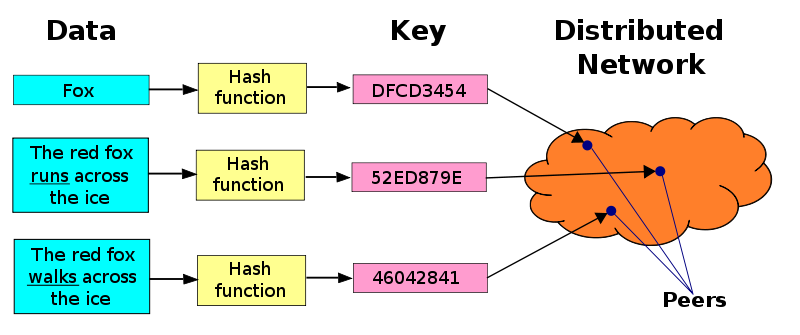
\includegraphics[width=0.5\textwidth]{images/DHT.png}
  \caption{\label{DHT}}
\end{figure}

So how do we map $hash(filename)$ to an actual node? 
In most DHTs, each node has a 160-bit identifier that determines which potential keys each node owns.\footnote{Keys and node IDs are 160 bits for consistency with the SHA-1 hash function. Nothing stops us from using a different hash function.}
Specifically, a node $n$ owns a key $k$ if $n$ is the closest node to $k$.
``Nearness'' is computed by a distance function $\delta(k, n)$, which varies depending on the DHT.

When deploying a distance function, one of the main considerations is load balancing.
Ideally, the keyspace is partitioned evenly between all the nodes in the network, so one node doesn't store more keys than another. If this is not the case, then that node can get bogged down, and the entire system will suffer in performance.

This form of consistent hashing ensures that when a node is added or removed from a system, only the keys owned by adjacent nodes are changed. 
When a node joins the system, it takes responsibility for some of its neighbor's keys.
When a node crashes or leaves the system, the keys mapping to the data it held must be allocated to new nodes.
Moreover, the more nodes are in a system, the fewer keys have to be remapped on every node entry or exit.
This is yet another advantage a DHT holds over a traditional hash table, which remaps its entire keyspace when a bucket is added or removed.



\subsection{Why Kademlia?}

\subsubsection{Unique Features}
There are many different kinds of DHTs out there. They differ in the size of their address space (128- or 160-bit keys?), in the type of hash function is used (SHA-1, SHA-2, etc.), in what gets hashed to produce keys (file names, file contents, etc.), in redundancy and reliability (nodes can dynamically agree to store the same key, just in case one them crashes), in the way traffic is routed, and in many other ways.

We opt for the Kademlia DHT, which has several unique features.
First, it requires minimal configuration.
When a node wants to join a network, little else is required of it than to perform a self-lookup.
By performing a query, the requester becomes aware of all the nodes that exist between it and the request's intended recipient.

Second, this frequently updated awareness affords nodes the ability to route their queries through low-latency paths.
And although knowledge spreads like the plague, there is a natural defense against denial of service attacks, since a node can only know about a limited number of other nodes.

Third, not only can Kademlia nodes select low-latency routes, but they can also send parallel asynchronous queries to avoid timeout delays.

Fourth, Kademlia features unidirectional routing, as opposed to bidirectional routing.
All node lookups and value lookups are guaranteed to converge on the same path, regardless of the requester.
Thus, caching key/value pairs along a path will reduce latency.
Unidirectionality is a consequence of using a symmetric distance function, namely \emph{bitwise exclusive or} (XOR).
That is, the distance function is denoted by $\delta(x,y) = x \oplus y$, and its property of symmetry is denoted by $\delta(x,y) = \delta(y,x)$.

\subsubsection{Node State}
Each Kademlia node stores a list for every bit in the address space, in this 160.
Think of these lists as a node's contacts or peers, and each element in the list stores a peer's IP, port, and node ID.
For $0 \leq i < 160$, list $i$ stores peers whose distance falls within the interval $[2^i, 2^{i+1})$.
That is, the $0^{\mathrm{th}}$ list stores peers that are 1 away; the $1^{\mathrm{st}}$ list, peers that are 2 or 3 away; the $2^{\mathrm{nd}}$ list, peers that are 4, 5, 6, or 7 away; and so on.

One of the biggest differences between Kademlia and other DHTs is that the keys are the hashed node IDs instead of hashed filenames or hashed file contents.
We use a Python implementation of the Kademlia DHT.



\section{Design Challenges}
\subsection{Replication}
\subsection{Synchronization}





\section{Implementation}
% implementation details

\subsection{Current Implementation}
% describe existing files, crypto, p2p, etc

\subsection{Additions}
% describe modifications to market, run, tornadoloop, etc

\subsection{Issues}




\section{Evaluation}




\section{Conclusion}



\end{document}
